Esta seção apresenta os detalhes da solução proposta pelo presente trabalho de conclusão de curso, descritas segundo o processo de AM \cite[vide Seção 1.5]{ref:marsland}. Na Seção  \ref{subsec:tarefa}, é apresentada a tarefa de aprendizado considerada, um passo a passo de como a solução proposta está caracterizada e alguns aspectos acerca da avaliação, tais como métrica de desempenho e técnica de validação cruzada. A base de dados experimentais utilizada neste trabalho é detalhada na Seção \ref{subsec:dados} e as tarefas de pré-processamento sobre a mesma são relatadas na Seção \ref{subsec:pre-process}. No tocante aos modelos de DL e seus parâmetros, os mesmos são apresentados na Seção \ref{subsec:modelos} . Por fim, a Seção \ref{subsec:resultados} contempla os resultados obtidos até o momento.

\subsection{Processo de Aprendizagem de Máquina} \label{subsec:tarefa}
No contexto deste trabalho, o problema da colorização de uma imagem será abordado como uma \emph{tarefa de regressão}, cujo objetivo é obter uma estimativa dos parâmetros de coloração dos pixels. De maneira mais detalhada, a Figura \ref{fig:aprendizado} ilustra o conjunto de passos a ser realizado.

\begin{figure}[h]
	\centering
	\caption{Detalhamento do processo de aprendizado.}
	\label{fig:aprendizado}
	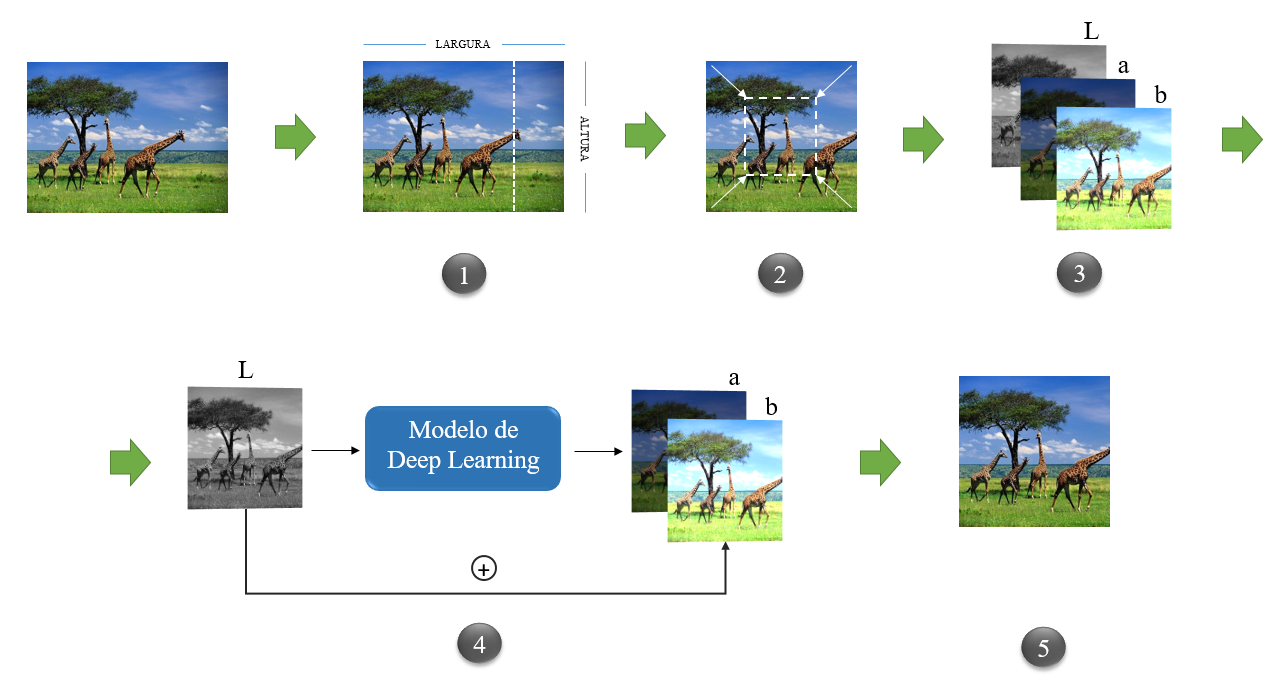
\includegraphics[width=0.95\textwidth]{./img/aprendizado}
\end{figure}

Dada uma imagem em tons de cinza que se deseja colorir, o primeiro passo a ser realizado (Passo 1) consiste no redimensionamento da imagem de acordo com a dimensão predominante (altura ou largura), com vistas a obter uma imagem quadrada. Em seguida, para que seja fornecida como entrada para os modelos de DL, a imagem será redimensionada para $128 \times 128$ pixels (Passo 2). Após esta etapa, o espaço de cores da imagem será convertido de RGB para CIELab (Passo 3). Desta conversão, o parâmetro de luminosidade $L$ será fornecido para o modelo de DL, cujo objetivo será produzir duas matrizes com os valores de coloração $a$ e $b$ (Passo 4). Por fim, a luminosidade $L$, já conhecida, será combinada com as matrizes de coloração $a$ e $b$ produzidas, compondo uma versão colorida da imagem inicial (Passo 5).

Para que os modelos propostos para realização da coloração produzam resultados factíveis, é necessária uma etapa de treinamento, em que imagens coloridas serão fornecidas sucessivamente às redes para ajustes dos pesos, produzindo mapas de características mais fidedignos ao domínio do problema. A base de dados a ser utilizada para esta etapa será descrita na seção a seguir.

No escopo deste trabalho serão consideradas as arquiteturas canônicas de CNNs VGGNet  e ResNet as quais serão ajustadas ao problema em questão mediante TL. Diferentes valores de parâmetros e hiperparâmetros (épocas, taxa de aprendizado, \emph{batch size}, etc.) serão considerados, sempre que possível, buscando um melhor ajuste do modelo ao problema em questão.

Nesta tarefa de regressão, realizada de acordo com o paradigma supervisionado, a métrica de desempenho utilizada será o Erro Quadrático Médio (MSE, do inglês \emph{Mean Squared Error}), definido como:

\begin{equation}
\textrm{MSE} = \frac{1}{n}\sum_{i=1}^n (y_i - \hat{y}_i)^{2}, \label{eq:mse}
\end{equation} em que $y_i$ é o valor real esperado para o exemplo $i$, $\hat{y}_i$ é o valor previsto pelo modelo para este exemplo e $n$ é o número de amostras presentes no conjunto de dados \cite{ref:faceli}.

O treinamento e testes das CNNs seguirão a abordagem \emph{Holdout} de validação cruzada, em que $70\%$ dos dados serão utilizados no treino e ajuste de parâmetros e o restante para avaliação, com vista a capturar a qualidade da generalização proposta pelos modelos considerados \cite{ref:brink}.


\subsection{Dados Experimentais} \label{subsec:dados}
Para alcançar os objetivos propostos no escopo deste trabalho de conclusão de curso, a base de dados a ser utilizada no processo de aprendizado será o conjunto de validação da tarefa \emph{Fine-grained classification} do ILSVRC $2012$ que está disponível em \cite{ref:image-net}. A Figura \ref{fig:visaogeral} apresenta uma visão geral deste conjunto de dados que dispõe de um total de $50$ mil imagens de diferentes naturezas, as quais foram coletadas do \emph{website} Flickr e de outras plataformas semelhantes e rotuladas manualmente por ausência ou presença de $1000$ diferentes categorias \cite{ILSVRC}. 

\begin{figure}[h]
	\centering
	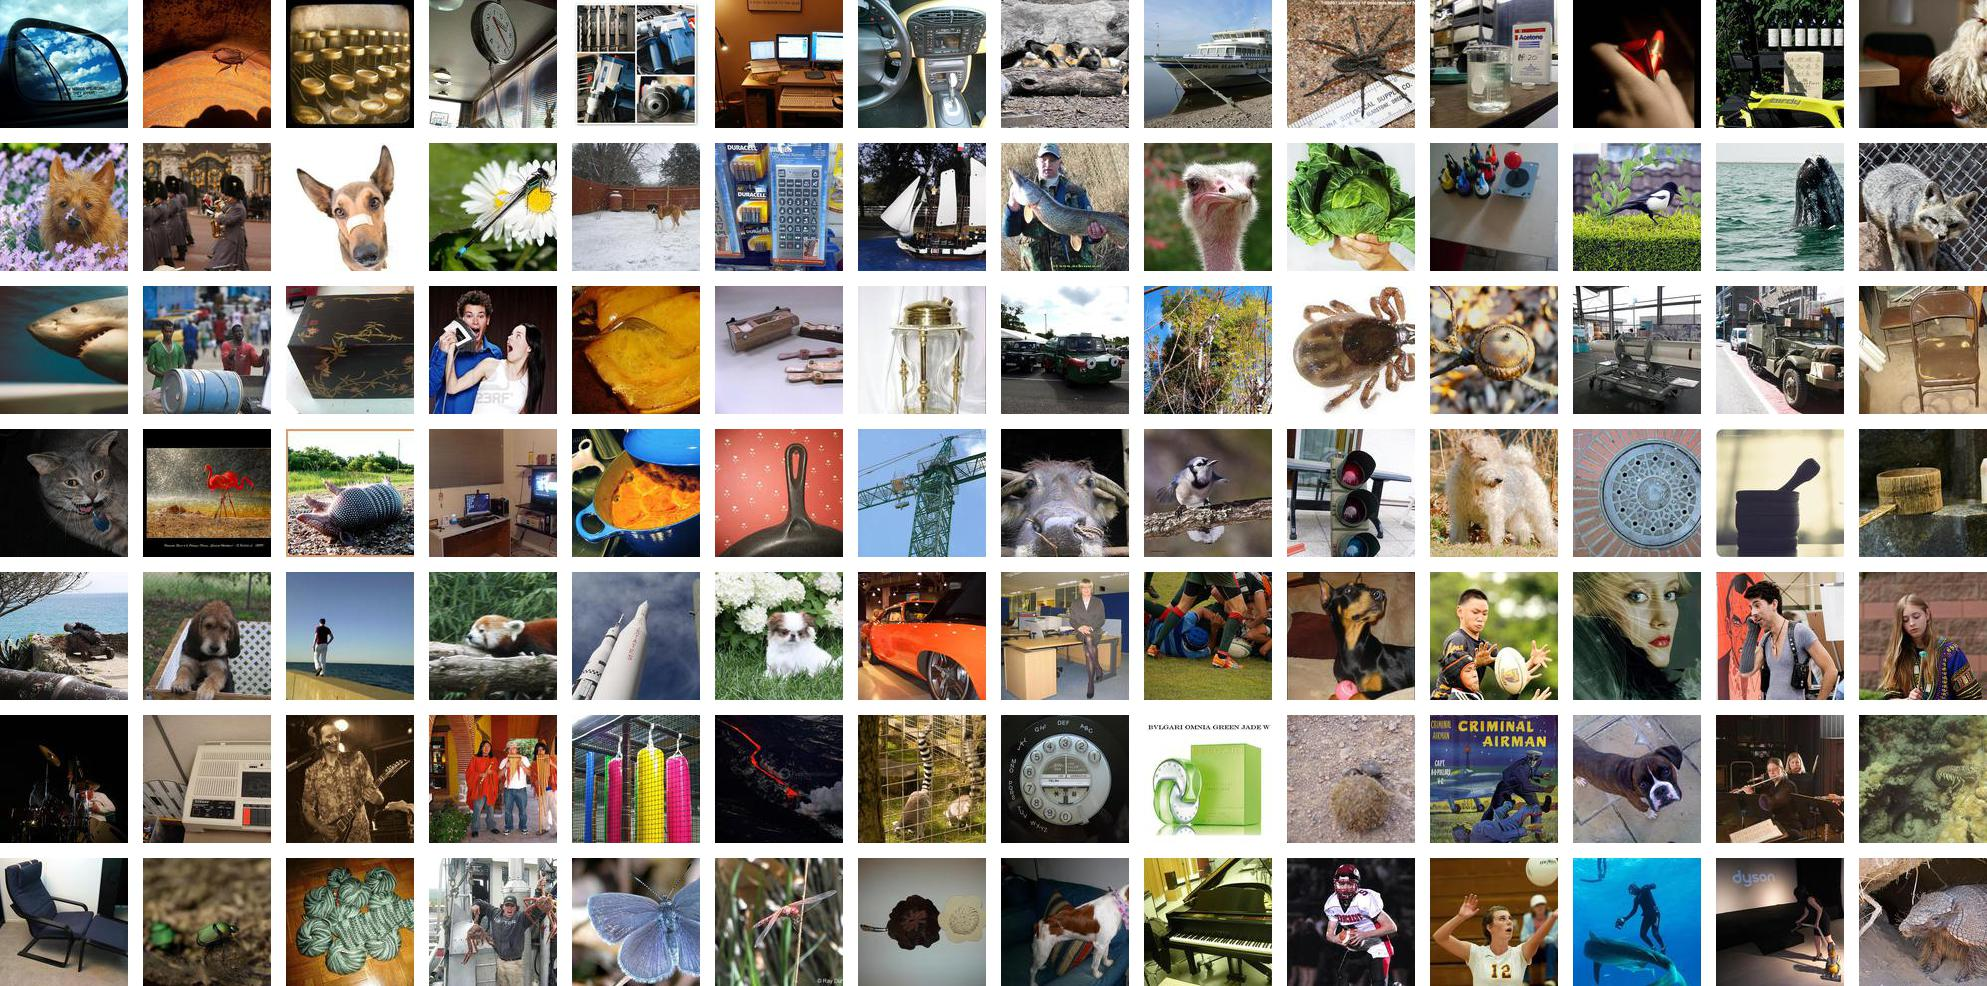
\includegraphics[width=1\textwidth]{./img/visaogeral}
	\caption{Visão geral do conjunto de dados.}
	\label{fig:visaogeral}
\end{figure}

Como dito anteriormente, conjunto de dados será particionado para compor o processo de aprendizado e desse modo $35$ mil imagens serão utilizadas para o treinamento e ajustes dos modelos e as outras $15$ mil para as análises de desempenho. Entretanto, antes de disponibilizar a base de dados para os modelos de DL, as imagens devem estar bem estruturadas e, portanto, devem passar por um pré-processamento, o qual será detalhado na Seção \ref{subsec:pre-process}.



\subsection{Limpeza e Pré-Processamento da Base de Dados} \label{subsec:pre-process}
Como se sabe, algoritmos de AM precisam de quantidades significativas de dados que estejam preferencialmente sem muitos ruídos. Entretanto, com o aumento do tamanho do conjunto de dados os custos computacionais também aumentam e faz-se necessário um pré-processamento desses dados para estruturá-los da maneira ideal sem que haja uma excessiva sobrecarga computacional \cite{ref:marsland}.

O conjunto de imagens que será utilizado no processo de colorização deste trabalho será submetido a um pré-processamento que se inicia padronizando a dimensão das imagens. Primeiramente, as imagens são redimensionadas de forma que possuam os mesmos tamanhos de largura e altura, para obtenção de uma imagem quadrada. Em seguida, cada imagem é redimensionada para $128 \times 128$ pixels, padronizando todas as imagens nesta mesma dimensão. Esta padronização visa tornar a tarefa de aprendizado factível diante dos recursos computacionais disponíveis.

Após a etapa de redimensionamento, a etapa seguinte consistiu em selecionar as imagens cujo espaço de cores fosse o RGB. Isto foi efetuado com o intuito de eliminar imagens em tons de cinza e em outros espaços de cores que demandassem um maior processamento posterior. No caso das imagens em tons de cinza, em particular, a eliminação das mesmas simplifica o processo de treinamento dos modelos, visto que estas não fornecem informação relevantes para aprendizado de colorações. Nesta etapa, foram eliminadas cerca de $900$ imagens que se encaixam em um dos critérios mencionados.

Em seguida, todas as imagens foram então convertidas do espaço de cores RGB para o espaço de cores CIELab, tendo em vista a diminuição dos parâmetros de entrada e saída no processo de aprendizagem e também a adequação aos procedimentos descritos na Seção \ref{subsec:tarefa}. Cada imagem passou então a corresponder a uma matriz de dimensões $3\times 128 \times 128$, a qual foi separada em duas partes: componente $L$, de dimensões $128 \times 128$, a ser fornecida como \emph{entrada} para os modelos, e componentes $a$ e $b$, a serem fornecidos como rótulo de \emph{saída} para o aprendizado supervisionado dos modelos, com dimensões $2 \times 128 \times 128$.


\subsection{Modelos e Parâmetros Considerados} \label{subsec:modelos}
Para o Passo 4, descrito na Seção \ref{subsec:tarefa}, será considerada a abordagem de TL, visando aproveitar parâmetros de redes CNNs pré-treinadas com \emph{datasets} massivos, especialmente o ImageNet. Para tanto, considerando a utilização do \emph{framework} \texttt{keras}, foi consultada a biblioteca de modelos previamente treinados, disponíveis no módulo \texttt{applications}. Como resultado, foram identificadas as arquiteturas canônicas e suas características elencadas na Tabela \ref{tab:cnns}.

\begin{table}[!ht]
	\caption{Arquiteturas canônicas e suas características disponíveis no módulo \texttt{keras.applications}.}
	\centering
	\begin{tabular}{c c c c}
		\toprule
		 Arquitetura & Profundidade & Parâmetros & Tamanho \\
		\midrule
		Xception & 126 & $22,910,480$ & 88 MB \\
		VGG16 & 23 & $138,357,544$ & 528 MB \\
		VGG19 & 26 & $143,667,240$ & 549 MB \\
		ResNet50 & 168 & $25,636,712$ & 99 MB \\
		InceptionV3 & 159 & $23,851,784$ & 92 MB \\
		InceptionResNetV2 & 572 & $55,873,736$ & 215 MB \\
		MobileNet & 88 & $4,253,864$ & 17 MB \\
		\bottomrule
	\end{tabular}

	\label{tab:cnns}
\end{table}

É interessante notar que todos estes modelos disponíveis foram pré-treinados com a base de dados do ImageNet. Considerando a quantidade de imagens e a variedade desses exemplos, acredita-se que estes pesos podem contribuir positivamente para o problema da coloração dada a transferência de aprendizado.

Levando em conta os recursos computacionais disponíveis em nuvem para este projeto e o tempo de processamento, duas CNNs, a VGG16 e ResNet50, disponíveis no \texttt{keras.applications} serão ajustadas perante TL para a tarefa de coloração proposta. Havendo tempo posterior disponível, outras arquiteturas também serão contempladas.

Dessas redes pré-treinadas, as últimas camadas serão substituídas por camadas completamente conectadas com saída compatível com as matrizes $a$ e $b$ de coloração. Eventuais re-treinos serão efetuados para ajuste de interconexão dessa nova camada. Serão consideradas $100$ épocas para o treinamento dos modelos propostos e os demais parâmetros terão seus valores padrões preservados.


\subsection{Resultados Parciais}
\label{subsec:resultados}
Todas as atividades inicialmente propostas na metodologia foram executadas conforme proposto no cronograma, sem descumprimento aos prazos inicialmente estabelecidos. Como resultado, destaca-se a descrição do problema segundo a perspectiva de uma tarefa de AM utilizando as técnicas de TL e DL.

Inicialmente, toda a base de dados foi consolidada e pré-processada conforme descrito na Seção \ref{subsec:pre-process} visando estruturar os dados para apresentá-los às CNNs. Este procedimento foi realizado utilizando a infra-estrutura de \emph{hardware} disponibilizada pela plataforma Google Cloud.

Preliminarmente, utilizando o método de validação cruzada \emph{holdout} com $70\%$ dos dados para treinamento, o modelo de arquitetura VGGNet16 pré-treinado com imagens do ImageNet foi a base para o TL realizado em um modelo treinado com uma pequena porcentagem do conjunto de dados para fins de testes. O treinamento foi executado em uma instância de máquina virtual da plataforma Google Cloud e obteve um tempo de execução de aproximadamente 6 minutos obtendo um MSE de $261,175$. O modelo foi treinado durante $3$ épocas, com uma taxa de aprendizado de $10^{-4}$ e todos os outros parâmetros preservados. Mais épocas e parâmetros serão considerados nas fases posteriores deste trabalho.




%\subsection{Análise Comparativa} \label{sec:analise}
%\input{./files/solucao/analise}
